\documentclass{standalone}
\usepackage{tikz}
\begin{document}
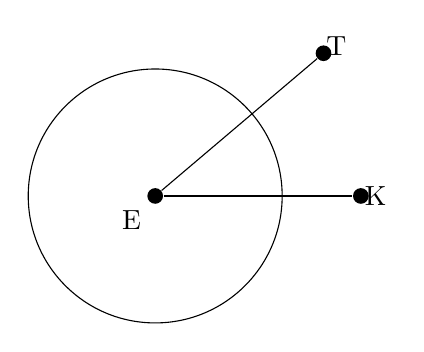
\begin{tikzpicture}
  \draw (0,0) node[circle,fill,inner sep=2pt] (E) {};
  \draw (2.6116,0) node[circle,fill,inner sep=2pt] (K) {};
  \draw (2.1375,1.8125) node[circle,fill,inner sep=2pt] (T) {};
  \draw (E) -- (K);
  \draw (E) -- (T);
  \draw (0,0) circle (1.6125cm);
  \node at (-0.3,-0.3) {E};
  \node at (2.8,0) {K};
  \node at (2.3,1.9) {T};
\end{tikzpicture}
\end{document}